the first step we need to take is analyzing the effect of varying a trajectory first. In general, one can expect to vary trajectory followed by the state of a control system in two ways: given a control, varying the initial conditions or, given the initial conditions, varying the control. Nevertheless it is still necessary to develop some tools to \textit{describe} the variation of the trajectory in some ways. 

\subsection{Variations and adjoint response}
\paragraph{Variational and adjoint equations}\mbox{}\\
Given a control system \controlSystem and am admissible control $\mu:I\fd U$ we have
\lista{
	\item the \grass{variational equation}  equation for $\Sigma$ with control $\mu$ is the differential equation
	\begin{multiLineSingleNumber}
		\statotdot=f(\statot,\mut);\\
		\dot{v}(t)=\Dderarg{1}f(\statot,\mut)\cdot v(t)\\
		(\statot,\mut)\in(\chi\times\R^n)
		\label{variational-equation}
	\end{multiLineSingleNumber}	
	
	
	\item the \grass{variational equation}  equation for $\Sigma$ with control $\mu$ is the differential equation
	\begin{multiLineSingleNumber}
		\statotdot=f(\statot,\mut);\\
		\lambdatdot=-\Dderarg{1}f^T(\statot,\mut)\cdot v(t)\\
		(\statot,\lambdat)\in(\chi\times\R^n)
		\label{adjoint-equation}
	\end{multiLineSingleNumber}
}

\subparagraph{interpretation} It is straightforward to see that the variational equation describes, through a linearization,  the evolution in time of a small (infinitesimal) variation from the original trajectory $\statot$, which is one of the solutions to the equation \ref{e1.1}.\\
Obviously, it is hoped that, given a certain control and initial condition, the solution to \ref{e1.1} is unique, but a-priori it cannot be said.\\
The geometrical interpretation of the adjoint equation is more subtle, but, in a naive way, one could say that, given an optimal trajectory, the adjoint response is a vector orthogonal to the hyerplane given by (directions of the )the possibile (infinitesimal) variations to that trajectory. 

\subsection{Variation and infinitesimal variation}
\paragraph{Definitions}\mbox{}\\
Let \controlSystem be a control system, $x_0\in\chi$ be an initial condition for eq. \ref{e1.1}, $\tzto\subset\R$ a time interval, $\mu\in\admContr{x_0,t_0,\tzto}$. a \grass{variation} of the trajectory \trajWinCond{\cdot} is map $\sigma:J\times\tzto\fd\chi$ with the following properties 
\lista{
	\item $J\subset\R;0\in int(J)$ is an interval for which zero reside in its internal part
	\item $\sigma(0,t)=$\trajWinCond{t} for each $t\in\tzto$
	\item $s\fd\sigma(s,t)\text{is of class }C^1\text{for each }t\in\tzto$
	\item $t\fd\sigma(s,t$ is a solution of eq. \ref{e1.1}.
}

Given a variation and it's relative "original" trajectory, there is another important quantity, which is he corresponding \grass{infinitesimal variation}. This is yet another map defined with the following limit
\equaz{
	\delta\sigma(t)=\frac{d}{ds}\bigg\rvert _{s=0}\sigma(s,t).
	\label{infinitesimal-variation-definition}
}
\begin{figure}[H]
	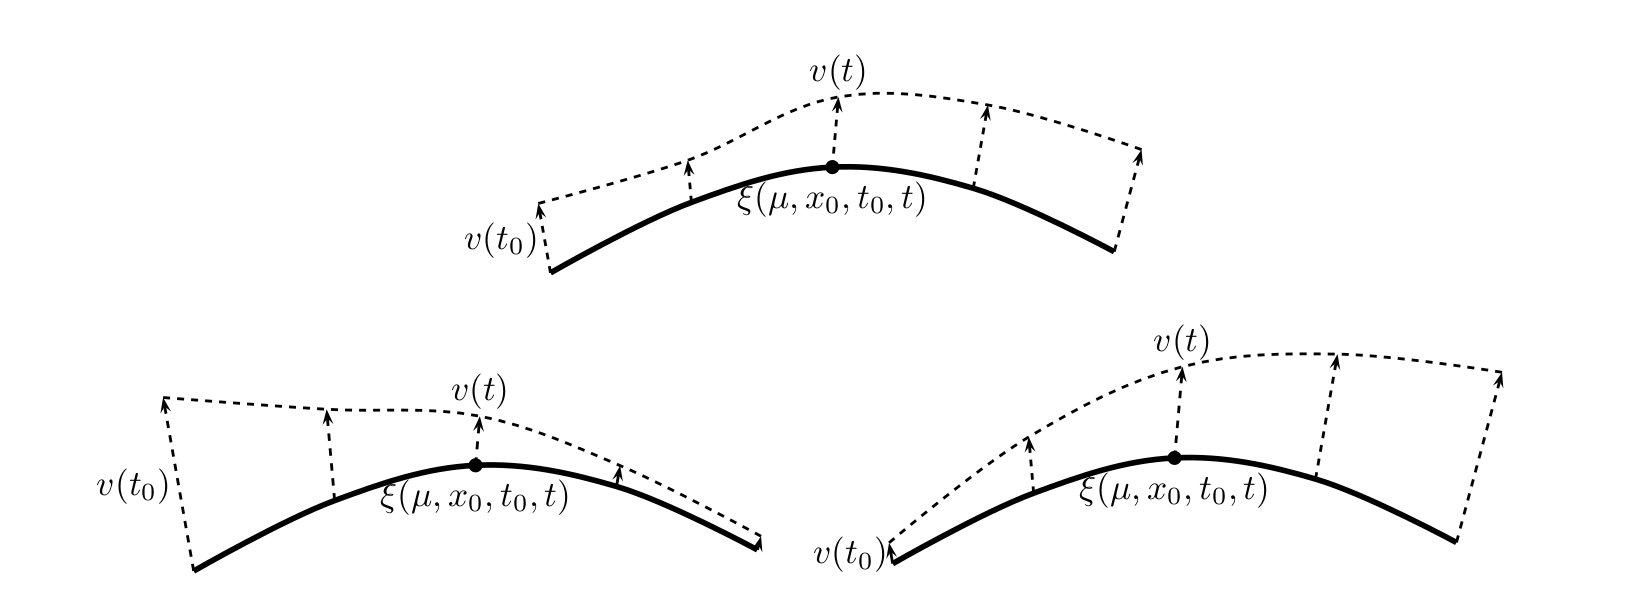
\includegraphics[width=\linewidth]{imgs/variations.png}
	\caption{}
	\ref{fig-variations}
\end{figure}
The dotted arrow represent the difference between the variation (at various times and at a given s), and the "original" trajectory, at the same time. The infinitesimal variation is then represented by a vector such that, at a given time $\overline{t},\sigma(s,\overline{t})\approx$\trajWinCond{\overline{t}}$+\delta\sigma(\overline{t})*s$
Actually, there is another interpretation to the image, in which the dotted arrow are the vectors represent the \grass{infinitesimal} variations, and the dotted line is just the envelope of the dotted arrows calculated at different times. In this case, the dotted part and the continuous-line of the figure have scales that have nothing to do one with each other. Nevertheless, in both interpretations, it is possible to understand the concept of a stable, unstable and "indifferent" trajectory, in which a disturbance in the trajectory is amplified rather than muted.
\paragraph{A theorem about infinitesimal variations} 
Here it will be stated that if a map is solution of equation \ref{variational-equation} then it is an infinitesimal variation , and vice versa.\\
Let \controlSystem be a control system, $x_0\in\chi$ be an initial condition for eq. \ref{e1.1}, $\tzto\subset\R$ a time interval, $\mu\in\admContr{x_0,t_0,\tzto}$. Given a map $v:\tzto\fd\R^n$ the statements \lista{
	\item there exists a map $\sigma$ which is a variation of \trajWinCond{\cdot} such that $v=\delta\sigma$;
	\item $t\fd($\trajWinCond{t}$,v(t))$ satisfies the variational equation \ref{variational-equation}.
}
are equivalent. 

\subparagraph{The foundamental matrix $\Phi$} During the demonstration of the preceding theorem, an $n\times n$ linear map $\Phi(t):\R^n\fd\R^n$ has been defined, as a map such that $\Phi(t)\cdot=\Dderarg{2}$\trajWinCond{t}$\cdot w$. \\
By differentiation one can see that $\Phi(t)$ sathisfies this matrix differential initial value problem:
\begin{gather*}
\dot{\Phi}(t)=\Dderarg{1}f(\trajWinCondMath{t},\mut)\circ;\text{   	   }\Phi(t_0)=Id_{n\times n} 
\end{gather*}

We thus define $\boldsymbol{\fondMatMath{\tau}{t}} $ as the solution to the matrix initial value problem 
\begin{equation*}
	\dot{\Phi}(t)=\Dderarg{1}f(\trajWinCondMath{t},\mut)\circ;\text{   	   }\Phi(\tau)=Id_{n\times n} ...
\end{equation*}

The importance of this matrix resides in the fact that, being the variational equation \ref{variational-equation} a linear one and being $\Phi$ the foundamental matrix of the equation, it is true that, for a variation $v(t)$ (which is also a solution to the variational equation, because of the theorem), $v(t)=\fondMatMath{t_0}{t}\cdot v(t_0)$\\
$\Phi$ also has some properties, about the composition of the 

\subsection{Properties of adjoint repsonse }
\paragraph[prop 4.4]{Hamilton's and adjoint equation}
\paragraph[prop 4.5]{Adjoint response and variations}
\subparagraph[4.6]{A corollary}
\paragraph[prop 4.7]{Foundamental matrix for the adjoint response}
\subsection{Needle variations}